\documentclass[output=paper]{langsci/langscibook} 
\author{Carina Steiner\orcid{}\affiliation{University of Bern, Center for the Study of Language and Society}}
\title{The dynamics of young learners’ L2 motivation: A longitudinal perspective}
\abstract{Affective dispositions in language learning are regarded as dynamic constructs that change over time. Yet, longitudinal studies in this field are relatively rare. In order to better understand these changes, this chapter reports a study that investigates the development of 578 primary school students’ English and French learning motivation, self-concepts, anxiety, and perceived support of teachers and parents at three measurement times over two academic years. While no drastic overall changes could be identified in our data, affective dispositions remain constantly higher for English than for French. Whereas students maintain their strong English-related motivations and self-concepts and English learning anxiety remains on a low level, French-related intrinsic motivation and self-concepts weaken with a parallel growth of anxiety. With regard to extrinsic motivation, both in leisure and school contexts, as well as perceived teacher and parental encouragement, a slight decrease is observed in both target languages.

These results are discussed with regard to previous findings and in light of the relation between English as a global lingua franca and French as a local foreign language.}
\IfFileExists{../localcommands.tex}{
  \addbibresource{localbibliography.bib}
  % add all extra packages you need to load to this file

\usepackage{tabularx,multicol}
\usepackage{url}
\urlstyle{same}

\usepackage{listings}
\lstset{basicstyle=\ttfamily,tabsize=2,breaklines=true}

%\usepackage{langsci-optional}
\usepackage{langsci-lgr}
\usepackage{langsci-gb4e}
\usepackage{langsci-optional}

\usepackage{enumitem}
\usepackage[group-digits=false, detect-weight=true]{siunitx}

\usepackage{todonotes}

  \newcommand*{\orcid}{}
 
  %% hyphenation points for line breaks
%% Normally, automatic hyphenation in LaTeX is very good
%% If a word is mis-hyphenated, add it to this file
%%
%% add information to TeX file before \begin{document} with:
%% %% hyphenation points for line breaks
%% Normally, automatic hyphenation in LaTeX is very good
%% If a word is mis-hyphenated, add it to this file
%%
%% add information to TeX file before \begin{document} with:
%% %% hyphenation points for line breaks
%% Normally, automatic hyphenation in LaTeX is very good
%% If a word is mis-hyphenated, add it to this file
%%
%% add information to TeX file before \begin{document} with:
%% \include{localhyphenation}
\hyphenation{
affri-ca-te
affri-ca-tes 
Soa-res
scru-ti-ny
me-ta-cog-ni-tion
}

\hyphenation{
affri-ca-te
affri-ca-tes 
Soa-res
scru-ti-ny
me-ta-cog-ni-tion
}

\hyphenation{
affri-ca-te
affri-ca-tes 
Soa-res
scru-ti-ny
me-ta-cog-ni-tion
}
 
  \togglepaper[1]%%chapternumber
}{}

\begin{document}
\SetupAffiliations{mark style=none}
\maketitle 
%\shorttitlerunninghead{}%%use this for an abridged title in the page headers

\section{Introduction, theoretical remarks}

This chapter deals with a more detailed examination of the \textit{dynamics} of different motivational and related affective dispositions in language learning at the primary school level. More precisely, the focus is set on the long-term dynamics of intrinsic motivation, motivation to use the L2 as a lingua franca, leisure- and school-related extrinsic forms of motivation, the ideal L2 self, as well as current self-concepts, perceived teacher and parental encouragement, and foreign language learning anxiety. General theoretical and empirical underpinnings on these constructs can be consulted in Chapters 1 and 7 in this volume.

Researchers in the field of L2 motivation commonly agree on the fact that these constructs change – at least to a certain extent – over time. For example, \citet[11]{Gardner2007} suggests that, although not considered as personality traits, motivational dispositions are relatively stable, and yet “amenable to change under certain conditions”. \citet[65]{DoernyeiOtto1998} go further and define motivation in a general sense as “dynamically changing cumulative arousal in a person”. 

Related to the question whether this construct changes over time, the temporal perspective on motivation is crucial: While moment-by-moment experiences on the micro-level (e.g. motivational fluctuations during a specific task or task cycle) are prone to change, processes on the macro-level (e.g. general affective dispositions towards L2 learning or the L2 speech community) remain more stable over a longer period of time (\citealt{DoernyeiUshioda2011}: 6). This chapter aims to provide a long-term view on L2 motivation development and, thus, all subsequent discussions relate to motivational dispositions on the \textit{macro}{}-level which are less fluctuant than situational motivations on the micro-level. 

Even though the importance of various affective dispositions for the language learning process has been widely discussed, very few studies deal with their dynamics at an early age. This is due to the assumption that motivation, attitudes, and other affective dispositions are only emerging at a certain age and are therefore instable in younger learners (see e.g. \citealt{Gardner2006}, \citealt{Doernyei2009}). As \citet{Heinzmann2013} argues from a pedagogical perspective, this is exactly why more empirical research into young learners’ motivation and attitudes is needed:

\begin{quote}
[I]f young children’s motivation and attitudes are not yet stabilized, this means that they are still malleable and something can be done about negative motivational and attitudinal dispositions before they become firmly established. \citep[4]{Heinzmann2013}
\end{quote}

\section{Motivational dynamics at the primary school level}\label{sec:08:2}

Although various scholars have pointed out the need for investigating the dynamics of children’s language learning motivation and related affective dispositions (see e.g. \citealt{Cenoz2004}, \citealt{McGroarty2001}), there are only few studies with a longitudinal design enabling robust conclusions about developmental processes (see e.g. \citealt{MihaljevicDjigunovic2012} or \citealt{MihaljevicDjigunovicNikolov2019} for an overview). 

An insightful study for the Swiss context comes from \citet{Heinzmann2013}, who investigated primary school students’ English learning motivation and attitudes at three measurement points in 3\textsuperscript{rd}, 4\textsuperscript{th} and 5\textsuperscript{th} grade ($n=552$). Her results suggest that pupils started with a strong motivation that remained relatively stable over the three measurement points. A closer examination of different subdimensions revealed that the biggest changes manifested in a slight drop of the intrinsic motivation from 3\textsuperscript{rd} to 4\textsuperscript{th} grade, while the motivation to use English as a lingua franca became continuously more important over time (cf. \citealt{Heinzmann2013}). Similar results in relation to instrumental motivation, which overlaps with Heinzmann’s lingua franca motivation, were also found by \citet{Nikolov2002} or, in a cross-sectional design, by \citet[256]{Tragant2006}.

Indices for an overall decline of motivation during primary school can be found in \citeauthor{BaderSchaer2005} (\citeyear{BaderSchaer2005}; see also \citealt{SchaerBader2003}, \citealt{Cenoz2004} for similar tendencies for children in the Basque country). In contrast, \citet[324]{PfenningerSingleton2016} show positive development tendencies for older students between 13 and 18 years of age. 

In addition to motivational changes, \citet[93]{Stoeckli2004} investigated the English self-concept of 133 pupils in a longitudinal perspective. His results suggest a decline after the 1\textsuperscript{st} grade, before re-strengthening until the end of 5\textsuperscript{th} grade. Stöckli argues that young children tend to overestimate themselves at the beginning of the learning process, but growing experience reassures the learners continuously (for a related discussion, see also \citealt{MihaljevicDjigunovicLopriore2011}: 50).

A longitudinal study by \citet{Henry2009} investigated young learners’ future self-concepts in the sense of Dörnyei's L2 motivational self system (e.g. \citealt{Doernyei2009}; cf. Chapter 1, \sectref{sec:01:4}). In Henry’s study, a motivation questionnaire was administered to Swedish students of English ($n=169$) after one and four years of instruction. While the results suggest a stable development for the entire sample, further analyses revealed different trajectories according to gender: whereas girls’ ideal self strengthened from 6\textsuperscript{th} to 9\textsuperscript{th} grade, it weakened for boys (cf. \citealt{Henry2009}: 184). 

As a final important factor, foreign language anxiety (cf. \citealt{MacIntyre1999}) is negatively related to persistence in foreign language learning.

Similar to the study by \citet{Henry2009}, a large-scale cross-sectional study by \citet{DewaeleEtAl2016} revealed gender effects related to foreign language anxiety. The results revealed that, across all age groups included in the analysis, girls tended to experience not only more positive, but also more negative emotions in foreign language learning. The authors conclude that this generally higher emotional activation in both negative and positive ways leads to more promising learning outcomes for girls than for boys (cf. \citealt{DewaeleEtAl2016}: 59).

\section{Motivational dynamics and the relation between English and French as foreign languages}

The discrepancy between motivation to learn English vis-à-vis other foreign languages has been widely discussed in Switzerland and beyond (see e.g. \citealt{BuylHousen2014}, \citealt{Ushioda2017}, \citealt{Busse2017}). Whereas the gap between English and French is discussed and supported by results in Chapter 7, the perspective in this chapter is developmental in nature. Scholars have repeatedly pointed out that pupils who have already learned English at school can lose their motivation to learn any other foreign language because, from an instrumental view, the global lingua franca serves well enough as a communication tool (see e.g. \citealt{Hufeisen2003}: 9, \citealt{MeissnerEtAl2008}: 109, \citealt{Ushioda2017}).

In the Swiss context, this concern has not been supported by empirical findings. In a quasi-experimental study carried out in Central Switzerland, no negative effect of previous English instruction on French learning motivation could be detected \citep{Heinzmann2010}. These results were supported by \citet[176]{BruehwilerLePapeRacine2017} who investigated motivational changes in relation to both English and French at the transition from primary to secondary school. 

With regard to the (in)stability of French- and English-related motivation, instrumental reasons referring to the aspiration for academic or professional success through language learning, were found to remain stable. Similar to \citet{Heinzmann2013}, a decline of intrinsic motivation was observed, with a parallel rise of motivation to use English as a lingua franca. The pattern was slightly different for French, where no growth of communication motivation could be identified (for a study with a similar age cohort in the UK, see \citealt{GrahamEtAl2016}).

In relation to foreign language anxiety, insights can be drawn from a longitudinal study conducted within a monitoring programme of the new foreign language curricula in regions at the French-German language border in Switzerland (cf. \citealt{SinghElmiger2017}). Questionnaire-based data collected between grade 5 and 8 revealed that, while children were continuously more satisfied with their English instruction, they felt much more stressed in French at the first data collection. Interestingly, stress levels tended to slightly lower for French and to increase for English over time. However, these results are to be interpreted cautiously because the sample changed between different measurement points and questionnaires were partly adapted.

\section{Motivational dynamics in the LAPS project}\label{sec:08:3}

As outlined above, there are few studies that investigate language learning motivation with a longitudinal design and even fewer with a focus on the relation between English and other, less prestigious foreign languages. As discussed in Chapter 7, Swiss children usually consider learning English more attractive than learning French. This leads us to define French as a less prestigious foreign language, at least in this particular context.

This chapter aims to provide additional insights by examining the dynamics of primary school students’ motivation, self-concept, anxiety, as well as perceived teacher and parental encouragement with regard to English and French learning at school.

The following research question is addressed: \textit{How do primary school students’ motivation, as well as associated affective dispositions, change over a period of two academic years with regard to English and French?}


\subsection{Participants and instruments}

In order to investigate the dynamics of affective dispositions, a total of nine scales from the pupil questionnaire in the LAPS II project administered in autumn 2017 (T1), spring 2018 (T2), and spring 2019 (T3) are analysed. A total of 578 datasets are included in the analysis (detailed information on participants can be consulted in Chapter 2, \sectref{sec:02:4}, in this volume; the sample size deviates from the overall data due to the exclusion of native speakers of English and/or French and due to missing questionnaire data of some pupils). 

At T1, students were at the beginning of grade 4 (cohort 4, $n=273$) and grade 5 (cohort 5, $n=305$). At T2, they were at the end of grade 4 and 5, and at T3 at the end of grade 5 and 6, respectively. Due to the integration of two age cohorts, the measurement points are partly overlapping in relative terms of school years. \tabref{tab:08:1} displays this overlap.

\begin{table}\small
% \begin{tabular}{lllllll}
% \lsptoprule
% Cohort 4 & T1: beginning of 4\textsuperscript{th} grade & T2: \\
% end of 4\textsuperscript{th} grade &  & T3: \\
% end of 5\textsuperscript{th} grade &  & \\
% Cohort 5 &  &  & T1: beginning of 5\textsuperscript{th} grade & T2: \\
% end of 5\textsuperscript{th} grade &  & T3: \\
% end of 6\textsuperscript{th} grade\\
% \lspbottomrule
\begin{tabularx}{\textwidth}{lQQQQQ}
\lsptoprule
Cohort 4 & T1: beginning of 4\textsuperscript{th} grade & T2:\newline end of 4\textsuperscript{th} grade &   & \cellcolor{black!20}T3:\newline end of 5\textsuperscript{th}   grade &    \\
Cohort 5 &    &   & T1: beginning of 5\textsuperscript{th} grade & \cellcolor{black!20}T2:\newline end of 5\textsuperscript{th}   grade & T3:\newline end of 6\textsuperscript{th} grade\\\lspbottomrule
\end{tabularx}
\caption{\label{bkm:Ref32572945}\label{tab:08:1}Overlap in measurement points between the two age cohorts in LAPSII}
\end{table}

\subsection{Questionnaires}

In the questionnaires related to affective dispositions, children were instructed to indicate for each item on a scale of 1 to 4 how strongly they agree with a certain statement.\footnote{1\,=\,maximum disagreement; 4\,=\,maximum agreement; see analysis report for a full description of all scales: \url{https://osf.io/r5ypz/}}

The English Questionnaire was administered at all three data collections. However, some items were not repeated based on a factor analysis at T1. For the calculation of summary scores, only items that were asked at all three measurement points were integrated. 

The French Questionnaire was administered at T2 and T3. Due to the fact that children in cohort 4 did not start French classes before T3, they were excluded from analyses related to French learning motivation.

Cronbach’s α were computed for all scales except for intrinsic motivation, which consists of two items only. The internal consistency was satisfactory for all scales (Cronbach’s α ranges between 0.67 and 0.91, cf. analysis report for detailed information, \url{https://osf.io/mc8jf/}).

\subsection{Data analysis}

The data were processed and analysed in R (R Core \citealt{Team2019}). Datasets and reports can be downloaded from OSF (\url{https://osf.io/mc8jf/}). Changes in affective dispositions over time were analysed in mixed effects models (package \textit{lme4,} \citealt{BatesEtAl2015}) that account for multiple measurements per student and allow for the test of potential class effects. For each affective subdimension, a model was fitted with the respective summary score as dependent variable. Group (cohort 4 and 5) and measurement point (T1, T2, T3) were entered as fixed effects. Random intercepts were entered for students and classes. Model assumptions were visually tested. In order to examine the relevance of the effects and potential interactions, a comprehensive model containing all effects and interactions was calculated and then compared to different reduced models via likelihood ratio tests (cf. \citealt{Winter2013}). 

\section{Results}
\subsection{L2 motivation, self-concepts, and anxiety}

The results of all final models related to English are summarised in \tabref{tab:08:2}  (cf. analysis report for full output of each model: \url{https://osf.io/r5ypz/}). The intercept indicates the predicted mean for cohort 4 at the first measurement point on a scale of 1 to 4. Estimates for the fixed effect \textit{group} indicate discrepancies between cohort 4 and 5 at T1, effects of \textit{measurement point} (T2 and T3) signal changes in the respective affective dimension over time. An interaction between group and measurement point was only revealed for intrinsic motivation, indicating different developments for the two age cohorts over time (cf. \figref{fig:08:1} and discussion below).

Between-subject variation and between-class variation is displayed under the respective random effect. The ideal L2 self was assessed at T2 and T3 only, and thus, the intercept indicates the predicted mean for T2.


\begin{table}
\begin{tabular}{l c *{3}{S[separate-uncertainty,table-format=-1.2(1)]}  cc}
\lsptoprule
{AD} & {Int.} & \multicolumn{3}{c}{Fixed effects (±SE)} & \multicolumn{2}{c}{Random effects}\\\cmidrule(lr){3-5}\cmidrule(lr){6-7}
&  & {Group} & \multicolumn{2}{c}{Measurement point}  & {School\footnote{$n=578$}} & {Class\footnote{$n=32$}}\\
&  & {Cohort 5} & {T2} & {T3} & {SD} & {SD}\\\midrule
IM & 2.78 & -0.08 +- 0.07 & 0.02 +- 0.05 & -0.11 +- 0.05 & 0.55 & \\
SM & 2.97 & -0.23 +- 0.07 & -0.13 +- 0.04 & -0.24 +- 0.04 & 0.53 & 0.16\\
LM & 2.65 & -0.12 +- 0.06 & -0.12 +- 0.04 & -0.18 +- 0.04 & 0.57 & \\
LFM & 3.26 & 0.09 +- 0.06 & 0.02 +- 0.03 & 0.04 +- 0.03 & 0.39 & 0.12\\
IS & 3.36 & 0.05 +- 0.06 &  & 0.02 +- 0.03 & 0.43 & 0.10\\
SC & 2.98 & 0.08 +- 0.05 & 0.01 +- 0.03 & 0.03 +- 0.03 & 0.53 & \\
AN & 2.09 & -0.13 +- 0.06 & -0.03 +- 0.03 & -0.02 +- 0.03 & 0.61 & \\
\lspbottomrule
\end{tabular}
\caption{Fixed and random effects for English motivation, self-concepts, and anxiety.\label{tab:08:2} AD: Affective dispositions, IM: Intrinsic motivation, SM: School motivation, LM: Leisure motivation, LFM: Lingua Franca motiation, IS: Ideal L2 Self, SC: L2 self-concept, AN: Anxiety, Int.: Intercept.}
\end{table}

\tabref{tab:08:3}  presents the results for changes in affective dispositions related to French for cohort 5 (as mentioned above, cohort 4 was excluded from these analyses because they didn’t attend French classes at T2). Estimates for \textit{measurement point} indicate changes in affective dispositions between T2 and T3. Between-subject and between-class variation is indicated under the respective random effects.

\begin{table}
\begin{tabular}{l c S[separate-uncertainty,table-format=-1.2(1)] c c}
\lsptoprule
{AD\footnote{Cohort 5 only.}} & {Int.} & {Fixed effects} & \multicolumn{2}{c}{Random effects}\\\cmidrule(lr){3-3}\cmidrule(lr){4-5}
   &      & {Measurement point} & Student\footnote{$n=305$} & Class\footnote{$n=19$}\\
   &      & {T3 (±SE)} & SD & SD\\\midrule
IM & 2.43 & -0.26  +-0.05 & 0.67 & \\
SM & 2.75 & -0.14  +-0.05 & 0.60 & \\
LM & 1.69 & -0.09  +-0.05 & 0.45 & \\
LFM & 2.69 & -0.17 +-0.05 & 0.53 & \\
IS & 2.78 & -0.27  +-0.04 & 0.57 & \\
SC & 2.53 & -0.16  +-0.04 & 0.56 & \\
AN & 1.97 & 0.13   +-0.05 & 0.59 & \\
\lspbottomrule
\end{tabular}
\caption{Fixed and random effects for French motivation, self-concepts, and anxiety\label{tab:08:3}. AD: Affective dispositions, IM: Intrinsic motivation, SM: School motivation, LM: Leisure motivation, LFM: Lingua Franca motiation, IS: Ideal L2 Self, SC: Current self-concept, AN: Anxiety, Int.: Intercept.}
\end{table}

All effects based on model predictions for intrinsic, school, leisure, and lingua franca motivation as well as for the ideal L2 self, the current L2 self-concept and anxiety are plotted in \figref{fig:08:1} (English) and \figref{fig:08:2}  (French).

As the data in \tabref{tab:08:2}  and \figref{fig:08:1} suggest, affective dispositions related to English remain relatively stable from the beginning of grade 4 until the end of primary school. The pupils start with a particularly strong lingua franca motivation and a high English self-concept, and these values even marginally increase over time. The Ideal L2 Self, which was measured at T2 and T3, also starts out very high and remains stable over the course of a school year. English learning anxiety, in contrast, remains on a low level, even decreasing slightly over time. In contrast, extrinsic motivations related to school and leisure activities are less stable, they weaken for both age cohorts from T1 to T3.

The only dimension where an interaction between group and measurement point could be identified is the intrinsic motivation: While this motivation steadily strengthens for cohort 5, it grows slightly for cohort 4 between the first and second measurement, before dropping again by T3. 

While a certain between-subject variation could be identified, the analysis revealed no considerable class effects.

\begin{figure}
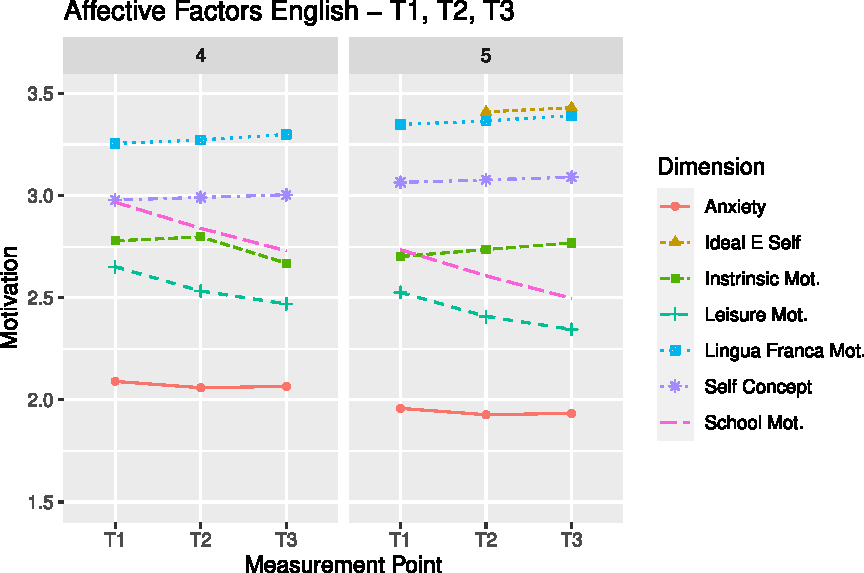
\includegraphics[width=\textwidth]{figures/Fig8.1.pdf}
\caption{Dynamics of affective dispositions related to English\label{fig:08:1}}
\end{figure}

\begin{figure}
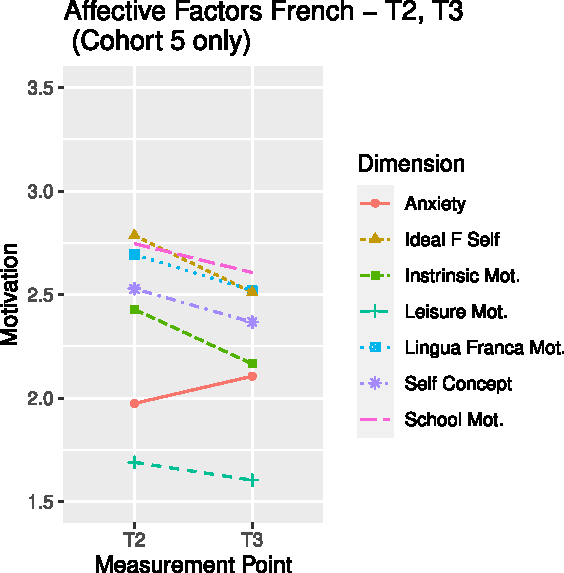
\includegraphics[width=.5\textwidth]{figures/Fig8.2.pdf}
\caption{Dynamics of affective dispositions related to French\label{fig:08:2}}
\end{figure}

With regard to French as the second foreign language, \tabref{tab:08:3}  and \figref{fig:08:2}  suggest a rather different situation. L2 motivation and its antecedents seem less stable than in English. In addition, students generally start with lower motivation and self-concepts at T2, and, at the same time, foreign language anxiety is somewhat higher than in English. Over the course of one school year, students’ motivation and self-concepts weaken, whereas anxiety grows notably.

\subsection{Teachers and parents}

Analogous to the motivation scales, an identical questionnaire for teacher and parental encouragement was administered in both English (T1--T3) and French (T2 and T3, cohort 5 only). \tabref{tab:08:4}  summarises all effects in relation to perceived teacher and parental encouragement in the two target languages. Fixed effects are plotted in Figures~\ref{fig:08:3}  and~\ref{fig:08:4}. No interactions between group and measurement point were identified.


\begin{table}
\fittable{\begin{tabular}{l c *{3}{S[separate-uncertainty,table-format=-1.2(1)]} cc}
\lsptoprule
& {Int.} & \multicolumn{3}{c}{Fixed effects (±SE)} & \multicolumn{2}{c}{Random effects}\\\cmidrule(lr){3-5}\cmidrule(lr){6-7}
      &      & \multicolumn{2}{c}{Measurement point}  & Group & Student\footnote{$n=578$} & Class\footnote{$n=32$}\\
      &      & {T2}          & {T3}          & {cohort 5}   & SD & SD\\\midrule
EN TE & 3.27 & -0.08 +-0.03  & -0.30 +-0.03  & 0.06 +-0.08  & 0.34 & 0.25\\
EN PE & 2.95 & -0.12 +-0.04  & -0.27 +-0.04  & 0.02 +-0.05  & 0.50 & \\
FR TE & 2.97 &               & -0.47 +-0.05  &              & 0.51 & 0.30\\
FR PE & 2.71 &               & -0.13 +-0.05  &              & 0.59 & \\
\lspbottomrule
\end{tabular}}
\caption{Fixed and random effects for perceived teacher and parental encouragement\label{tab:08:4}. EN: English, FR: French, TE: Teacher encouragement, PE: Parental encouragement, Int: Intercept.}
\end{table}

  
\begin{figure}
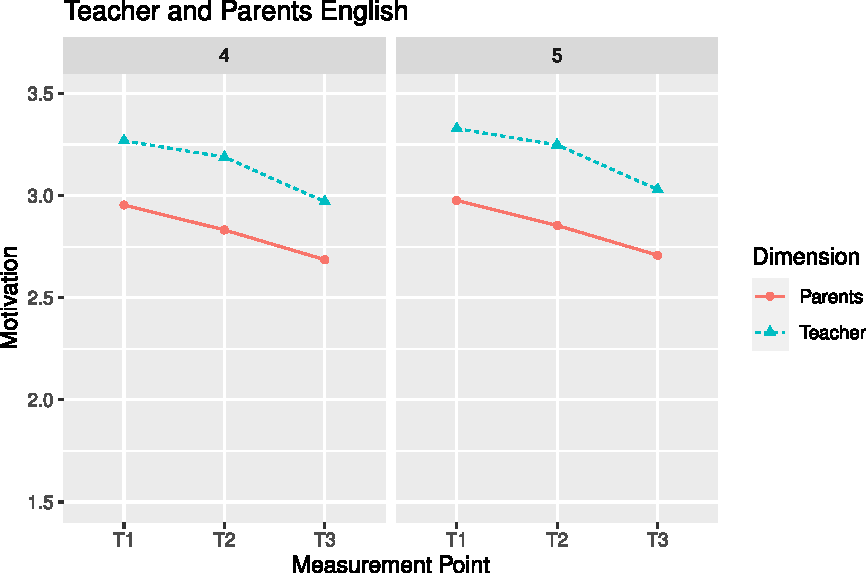
\includegraphics[width=\textwidth]{figures/Fig8.3.pdf}
\caption{Dynamics of perceived teacher and parental encouragement (English)\label{fig:08:3}}
\end{figure}

  
\begin{figure}
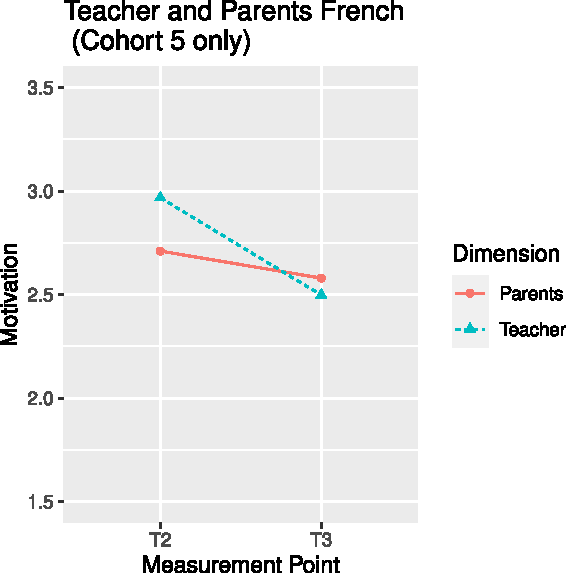
\includegraphics[width=.5\textwidth]{figures/Fig8.4.pdf}
\caption{Dynamics of perceived teacher and parental encouragement (French)\label{fig:08:4}}
\end{figure}

Our analysis revealed similar trajectories for both cohorts and target languages with regard to teacher and parental encouragement. While students in both cohorts perceive their L2 teacher and parents as very supportive and encouraging at the first measurement point, this perception weakens over time. In particular, this applies to the French teachers, where the strongest drop was observed. Additionally, considerable between-class variation in both languages was revealed in relation to perceived encouragement by the L2 teacher (cf. analysis report, p. 26: \url{https://osf.io/r5ypz/}).

\subsection{Gender effects}

On the basis of previous studies that suggest differences between girls and boys related to the development of foreign language anxiety and the Ideal L2 self, these two dimensions were subjected to further analyses and tested for potential gender effects. 

For both target languages, no gender effects were observed with regard to the Ideal L2 self. In contrast, models related to anxiety with gender as an additional fixed effect revealed that girls have higher levels of anxiety than boys. The effect was slightly stronger for English ($\beta_{\text{English}}=0.18$, $\text{SE}=0.06$; \newline
 $\beta_{\text{French}}=0.17$, $\text{SE}=0.09$). At the same time, gender did not interact with measurement point, which indicates that girls’ anxiety remains constantly higher than boys’. As pointed out by an anonymous reviewer, there could also be a reporting bias at play, with girls being more likely to admit to feeling anxious than boys.

\section{Discussion}

With reference to the research question stated in Section~\ref{sec:08:3} above, our results globally support previous findings in that primary school students’ motivation and related affective dispositions do not change drastically from middle to late primary school. Accordingly, the most obvious difference was not observed between different measurement points, but between the target languages: English motivation and self-concepts were both higher and more stable, whereas anxiety was lower than in French. Particularly, this applies to the intrinsic motivation, where our results are not entirely in line with previous findings (cf. \citealt{Heinzmann2013}, \citealt{BruehwilerLePapeRacine2017}). Whereas intrinsic reasons for foreign language learning remain rather positive for English, they are comparatively low for French and even weaken by the end of primary school.

Another result worth highlighting concerns L2 anxiety: Whereas it does not change for English, it intensifies for French. This contradicts previous findings which observed a decline of perceived stress in French classes over time (cf. \citealt{SinghElmiger2017}). With regard to gender effects, our data support findings by \citet{DewaeleEtAl2016} and indicate constantly higher levels of anxiety for girls than for boys in both French and English classes.

Low motivation levels were also identified with regard to the use of English and French in the students’ leisure time. The results suggest that pupils do not see much use of these languages for computer games, consulting information on the internet, or understanding the lyrics of their favourite music. The reason therefore could be related to the fact that English and French computer games, songs, or websites are not highly important for young learners at the beginning of their foreign language learning process. This is in line with findings from \citet{Heinzmann2013}.

A similar development pattern for both languages was also observed for school-related extrinsic motivation and perceived teacher and parental encouragement, which were rather high at the beginning, but decreased somewhat over time in French as well as in English. This might be due to the fact that pupils become more and more independent of adults and learning languages in order to profit academically becomes less important. In addition, the only notable between-class variation was detected for perceived teacher support. This underpins the critical role of the teacher which is also discussed in Chapters 3 and 7. 

Encouraging results could be identified with respect to the ideal L2 self and the lingua franca motivation. The values are particularly high in English, but they are positive and stay above the scale mean in French, too. This supports findings by \citet{Heinzmann2013} and suggests that children believe that they will become competent users of these languages and that the direct application of their language skills in order to communicate with English- or French-speaking people is strongly and steadily endorsed. Contrary to \citet{Henry2009}, our analyses revealed no gender effect related to ideal L2 selves. However, Henry’s study gives reason to expect that such effects might become apparent with increasing age, as the ideal L2 self is not yet stable at an early age and is expected to become more pronounced over time (cf. also \citealt{Doernyei2009}).

\section{Conclusion}

Our study is based on a quantitative analysis of longitudinal questionnaire data from a relatively large sample. It would be insightful to complement our findings with qualitative measures (such as semi-structured interviews and observations) in a mixed-methods approach. Furthermore, collecting data at critical moments in the learning process (such as shortly before starting, and at transitions between school types) would provide an additional perspective. Considering these aspects in future studies would allow for a more thorough understanding of how pupils' affective dispositions develop.

These restrictions considered, some general conclusions can be drawn from the results presented in this chapter. Firstly, while there are no drastic changes, primary school pupils have much more promising motivation profiles with regard to English than with regard to French: English learning motivation is stronger, self-concepts are higher, and anxiety is lower than in French. Additionally, all these affective dispositions are more stable in English than in French, where they drop somewhat between the end of the first and second year of instruction. In contrast, the development of motivation regarding academic success, and perceived teacher and parental support proved to be independent of the target language. Our data suggest similar declines in these dimensions for both English and French. An interesting pathway for future studies related to contextual effects on young learners’ L2 motivation would be to focus on the perception of peer influence and assess to what extent individual students in a classroom affect their peers’ L2 motivation and self-concepts.


{\sloppy\printbibliography[heading=subbibliography,notkeyword=this]}
\end{document}
